\documentclass[11pt,class=report,crop=false]{standalone}
\usepackage[screen]{../mathgame}

\usepackage{siunitx}
%\sisetup{locale = FR,detect-all,per-mode = symbol}

\begin{document}

\newcommand{\Cl}{\operatorname{\it Cl}}

%====================================================================
\chapitre{Lumière}
%====================================================================

%
%\insertvideo{yUgpElITYTg}{partie 5.1. Bits classiques}
%
%\insertvideo{iET0snUXj0k}{partie 5.2. Portes logiques}
%
%\insertvideo{JKmC2u5kvKg}{partie 5.3. Algorithme et complexité}


\objectifs{Comment une scène est-elle éclairée ? Quelle est la couleur des objets illuminés ?}



%%%%%%%%%%%%%%%%%%%%%%%%%%%%%%%%%%%%%%%%%%%%%%%%%%%%%%%%%%%%%%%%%%%%%
\section{Physique de la lumière}

%--------------------------------------------------------------------
\subsection{Vue d'ensemble}

La lumière possède à la fois les propriétés d'une onde et des corpuscules (photons). La lumière et l'éclairage sont des phénomènes complexes, difficiles à modéliser. Ici nous allons faire des hypothèses simplificatrices :
\begin{itemize}
  \item L'éclairage est direct, avec une seule source lumineuse. Si on avait plusieurs sources, il suffirait de faire les calculs pour chaque source. Par contre on considère que les objets sont uniquement éclairés par les sources lumineuses et non par réflexion de la lumière sur d'autres objets (comme le serait l'éclairage via un miroir par exemple).

  \item Il n'y a pas de transparence. Un objet avec transparence réfléchit une partie de la lumière reçue et laisse passer une autre partie. Nos objets seront opaques.

\end{itemize}


\myfigure{0.8}{\tikzinput{fig-lumiere-01}}

Le but est de déterminer la couleur d'un objet perçu par un observateur (\oe{}il, caméra, capteur\ldots). Dans la pratique, on décompose l'objet en surfaces élémentaires (petits carrés ou petits triangles par exemple) et on détermine la couleur de chaque surface élémentaire.

Cette couleur dépend de la \emph{source lumineuse} (position, direction, intensité, couleur\ldots), de l'\emph{objet} observé (position, orientation, couleur, texture\ldots) ainsi que de la position de l'\emph{observateur}.

%--------------------------------------------------------------------
\subsection{Physique}

Le vocabulaire permet de distinguer ce qui est émis par la source lumineuse de ce qui reçu/perçu par l'objet/l'observateur.

\begin{itemize}
  \item \textbf{Luminosité}/Intensité lumineuse/Éclairage/\emph{Luminance}.\index{luminosite@luminosité}

  L'unité désuète d'intensité lumineuse est le \emph{watt} (exemple une ampoule classique de \SI{75}{\watt}, un projecteur de \SI{500}{\watt}). Cela correspondait à la puissance consommée par l'éclairage avant l'apparition des ampoules LED. L'unité officielle est le \emph{lumen} (lm) : elle compte le flux d'énergie lumineuse (puissance) pour un angle d'un stéradian.
  Exemple : l'éclairage d'une pièce de 10 ou \SI{15}{\meter^2} nécessite une intensité totale d'environ 3000 à \SI{5000}{\lumen}.  

  La luminosité c'est donc ce qui arrive vers l'objet, ce n'est pas ce qui est réfléchi et observé.

  \item\textbf{Illumination}/Éclairement/\emph{Illuminance}.\index{illumination}

  L'illumination c'est la façon dont la lumière arrive vers l'objet. Elle dépend des propriétés physiques de l'objet (position, orientation\ldots).
  L'unité d'éclairement est le \emph{lux} (lx) : c'est le flux d'énergie reçue par une unité de surface. Exemple : $1$ lumen illuminant une surface de \SI{1}{\meter^2} correspond à $1$ lux. 
\end{itemize}


%--------------------------------------------------------------------
\subsection{Couleur}

\index{couleur}

La lumière possède sa couleur propre, l'objet possède aussi sa couleur propre. Le but est d'attribuer une couleur perçue à (une surface élémentaire de) l'objet.

\begin{itemize}
  \item Une lumière monochromatique est caractérisée par une seule longueur d'onde : de \SI{400}{\nano\meter} (violet) à \SI{800}{\nano\meter} (rouge) pour les longueurs d'ondes visibles. C'est l'analogue de jouer une seule note de musique sur un piano.

  \item La lumière est une superposition d'ondes monochromatiques (comme un accord de musique où plusieurs touches sont jouées en même temps).

  \item L'objet absorbe certaines ondes (de longueurs d'onde déterminées) et en réfléchit d'autres. 
  Par exemple, si un objet, éclairé par une lumière blanche, absorbe le bleu et réfléchit le rouge et le vert alors sa couleur perçue sera jaune (= rouge + vert).
\end{itemize}

\medskip

Nous caractériserons une couleur via le système RGB (\emph{Red/Green/Blue}).
\begin{itemize}
  \item Une couleur est caractérisée par trois réels $(r,g,b)$ avec $r,g,b \in [0,1]$.
  Exemples : $(1,0,0)$ est la couleur rouge, $(1,1,0)$ est du jaune\ldots

  \item \textbf{Addition.} 
  L'addition de deux couleurs se fait terme à terme, sans dépasser $1$.
  C'est par exemple l'opération naturelle lorsque on considère l'éclairage total produit par deux sources lumineuses.
  Si $\Cl_1 = (r_1,g_1,b_1)$ et $\Cl_2 = (r_2,g_2,b_2)$ alors l'addition totale est $(r_1+r_2,g_1+g_2,b_1+b_2)$. Cependant il faut prendre garde à ce qu'aucune composante ne dépasse $1$. Ainsi l'addition de couleurs est définie par la formule :
  
  \smallskip

  \mybox{$\displaystyle \Cl_1 \oplus_{cl} \Cl_2 = \big( \min(r_1+r_2,1), \min(g_1+g_2,1), \min(b_1+b_2,1)\big)$}

  \item \textbf{Multiplication.}
  La multiplication s'effectue aussi terme à terme:
  
  \smallskip
  
  \mybox{$\displaystyle \Cl_1 \otimes_{cl} \Cl_2 = (r_1r_2, g_1g_2, b_1b_2)$}

  Lorsque une lumière de couleur $\Cl_1$ éclaire un objet de couleur $\Cl_2$, la multiplication des couleurs renvoie la couleur perçue.
  Exemple : si une lumière de couleur $\Cl_1 = (1,0,1)$ (violet) éclaire un objet de couleur $\Cl_2 = (1,1,0)$ (jaune) alors la multiplication des couleurs donne  
  $\Cl_1 \otimes_{cl} \Cl_2 = (1,0,0)$, ainsi la couleur perçue de l'objet est rouge.
  Pour la multiplication de couleurs sombres, on peut ajuster la formule par un facteur multiplicatif.
  
\end{itemize}


%--------------------------------------------------------------------
\subsection{Notations}

Introduisons les notations utilisées dans la suite du chapitre.



\myfigure{0.8}{\tikzinput{fig-lumiere-02}}

\emph{Trois points.}
\begin{itemize}
  \item $S$ : le point origine de la source lumineuse,
  \item $P$ : le point centré sur la surface élémentaire de l'objet,
  \item $O$ : le point où on place la caméra/l'\oe{}il/l'observateur.
\end{itemize}

\medskip
\emph{Trois vecteurs.}
\begin{itemize}
  \item $\vec \ell$ : le vecteur unitaire issu de $P$ dirigé \emph{vers} la source lumineuse,
  \item $\vec n$ : le vecteur unitaire orthogonal à la surface élémentaire,
  \item $\vec v$ : le vecteur unitaire issu de $P$ et dirigé vers l'observateur $O$.
\end{itemize}


%%%%%%%%%%%%%%%%%%%%%%%%%%%%%%%%%%%%%%%%%%%%%%%%%%%%%%%%%%%%%%%%%%%%%
\section{Éclairage}

\index{lumiere@lumière}

%--------------------------------------------------------------------
\subsection{Lumière directionnelle}

Les rayons lumineux arrivent tous avec la même direction. C'est le cas par exemple de la lumière du soleil, ou d'une source lumineuse très éloignée.

\myfigure{0.8}{\tikzinput{fig-lumiere-03}}

Cette lumière est caractérisée par :
\begin{itemize}
  \item une direction : si $\vec u$ est le vecteur qui indique la direction des rayons, alors 
$$\vec\ell = -\frac{\vec u}{\|\vec u\|}.$$
  \item une intensité : $i_\ell$.
\end{itemize}
L'intensité $i_\ell$ et cette direction $\vec \ell $ sont constantes, quelle que soit la position du point $P$.


%--------------------------------------------------------------------
\subsection{Lumière ponctuelle}

La lumière \og{}rayonne\fg{} dans toutes les directions depuis la source, comme par exemple une ampoule.


\myfigure{0.8}{\tikzinput{fig-lumiere-04}}

Le vecteur $\vec\ell$ dépend de la position du point $P$ :
$$\vec \ell = \frac{\overrightarrow{PS}}{\|\overrightarrow{PS}\|}.$$

L'énergie lumineuse $i_\ell$ reçue au point $P$ diminue lorsque $P$ s'éloigne de la source $S$. Selon quelle loi varie cette intensité ?
Notons $r = PS$ la distance entre le point $P$ et la source. Notons $i_0$ l'intensité reçue à une distance d'une unité (par exemple \SI{1}{\meter}).
\begin{proposition}
~
\mybox{$\displaystyle i_\ell = \frac{i_0}{r^2}$}
\end{proposition}

\emph{Justification.} Notons $E_0$ l'énergie lumineuse qui traverse une sphère de rayon $1$ centrée sur la source $S$ pendant une unité de temps (ex. \SI{1}{\second}). Cette énergie se répartit uniformément sur une surface d'aire $4\pi$ (rappel : l'aire d'une sphère de rayon $r$ est $4\pi r^2$). 


\myfigure{0.6}{\tikzinput{fig-lumiere-05}}

Un tout petit peu plus tard ces rayons traversent la sphère de rayon $r$. L'énergie $E_0$ est conservée mais cette fois se répartit sur une surface d'aire $4\pi r^2$. Ainsi chaque élément de surface reçoit beaucoup moins d'énergie.
Par exemple, \SI{1}{\meter^2} de la sphère de rayon $1$ reçoit une énergie $\frac{E_0}{4\pi}$, alors que \SI{1}{\meter^2} de la sphère de rayon $r$  reçoit une énergie $\frac{E_0}{4\pi r^2}$.

\bigskip

\emph{Variante avec plus de paramètres.} 
\mybox{$\displaystyle i_\ell = \frac{1}{\alpha r^2 + \beta r + \gamma}$}
Les paramètres $\alpha,\beta,\gamma$ permettent davantage de réglages pour obtenir un éclairage plus réaliste. Si $\alpha = \frac{1}{i_0}$, $\beta=0$, $\gamma=0$, on retrouve la loi précédente.

%--------------------------------------------------------------------
\subsection{Spot}

Pour un spot, les rayons lumineux rayonnent à partir de la source, mais sont limités par un cône.  Par exemple : un spot, une lampe de poche, un projecteur.

\myfigure{1}{\tikzinput{fig-lumiere-06}}

Le cône est caractérisé par un axe central $\vec u$ (supposé unitaire) et un demi-angle $\theta$.


\begin{proposition}
Le point $P$ appartient au cône de sommet $S$, d'axe $\vec u$ et de demi-angle $\theta$ si et seulement si :
\mybox{$\displaystyle \cos(\omega) \ge \cos(\theta)$}
où l'angle $\omega$ est l'angle de $P$ par rapport à l'axe du cône :
\mybox{$\displaystyle \cos(\omega) = -\vec \ell \cdot \vec u$}
\end{proposition}

\myfigure{1}{\tikzinput{fig-lumiere-07}}

\begin{proof}
Tout d'abord on obtient l'angle $\omega$ entre $\overrightarrow{SP}$ et $\vec u$ par la relation $\vec \ell \cdot \vec u = - \cos(\omega)$, donc :
$$\cos(\omega) = -\vec \ell \cdot \vec u.$$
De plus $P$ appartient au cône si l'angle $\omega$ est plus petit que l'angle $\theta$, plus précisément lorsque $|\omega| \le \theta$, ce qui équivaut à $\cos(\omega) \ge \cos(\theta)$. D'où le résultat.
\end{proof}

L'intensité lumineuse reçue par un point du cône suit la même loi que celle de la lumière ponctuelle :
\mybox{$\displaystyle
i_\ell = 
\begin{cases}
\frac{i_0}{r^2} & \text{si } \cos(\omega) \ge \cos(\theta) \\
0               & \text{sinon}
\end{cases}
$}
On rappelle que $r = SP$.


\myfigure{0.5}{
	\tikzinput{fig-lumiere-08}\qquad\qquad
    \tikzinput{fig-lumiere-09}
}

\myfigure{1}{\tikzinput{fig-lumiere-10}}

Pour atténuer le passage zone obscure/zone éclairée, on peut effectuer une transition douce au bord du cône. On assombrit  progressivement la zone éclairée située à angle $\omega$ lorsque celui-ci se rapproche de l'angle $\theta$, selon la formule :
\mybox{$\displaystyle
i_\ell = 
\begin{cases}
\frac{i_0}{r^2} \left(\cos(\omega)\right)^{e_\text{att}} & \text{si } \cos(\omega) \ge \cos(\theta) \\
0               & \text{sinon}
\end{cases}
$}
L'exposant d'atténuation $e_\text{att}$ permet de paramétrer cette transition, qui est plus condensée pour des petites valeurs de l'exposant.

\begin{center}
	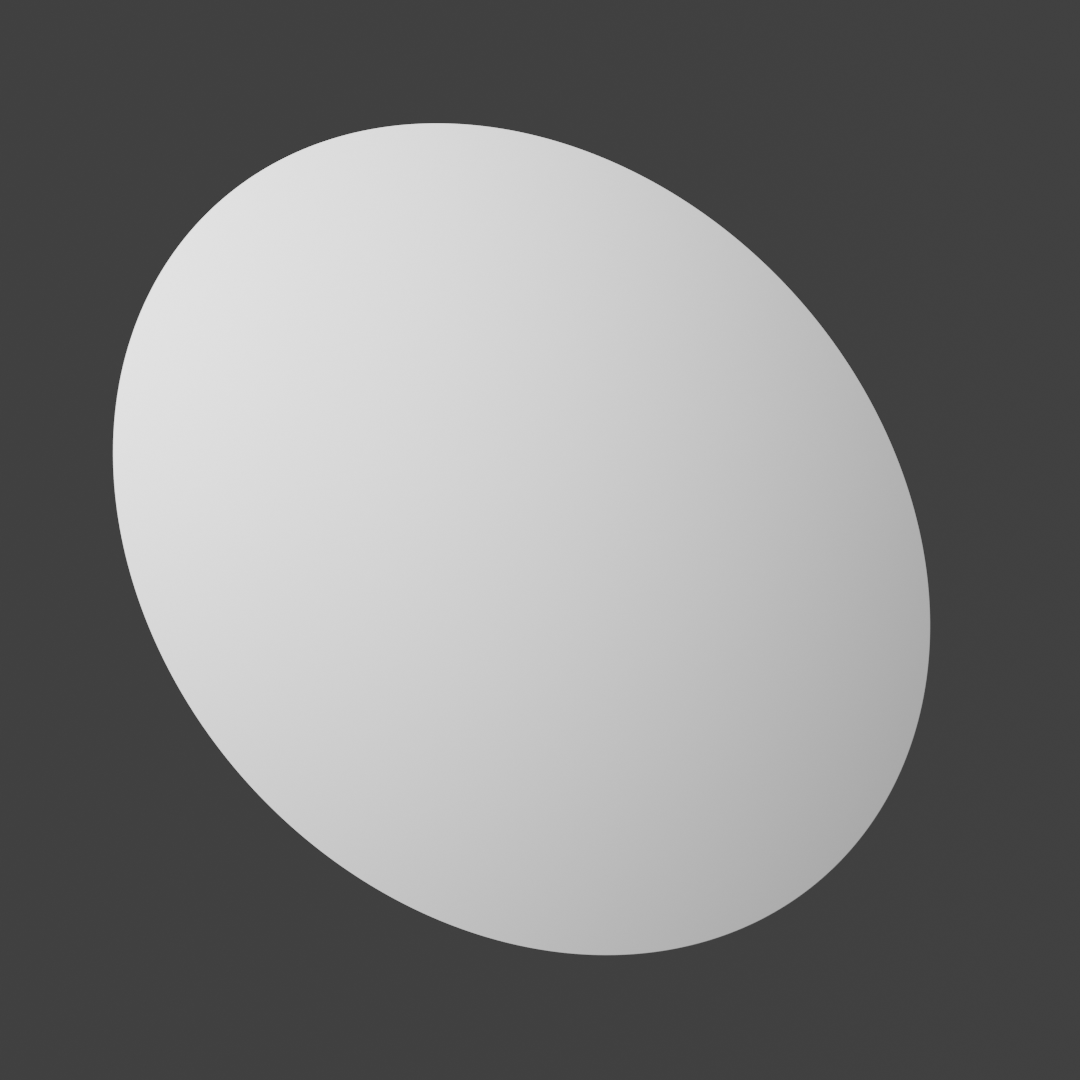
\includegraphics[scale=\myscale,scale=0.1]{figures/spot-01}\quad
	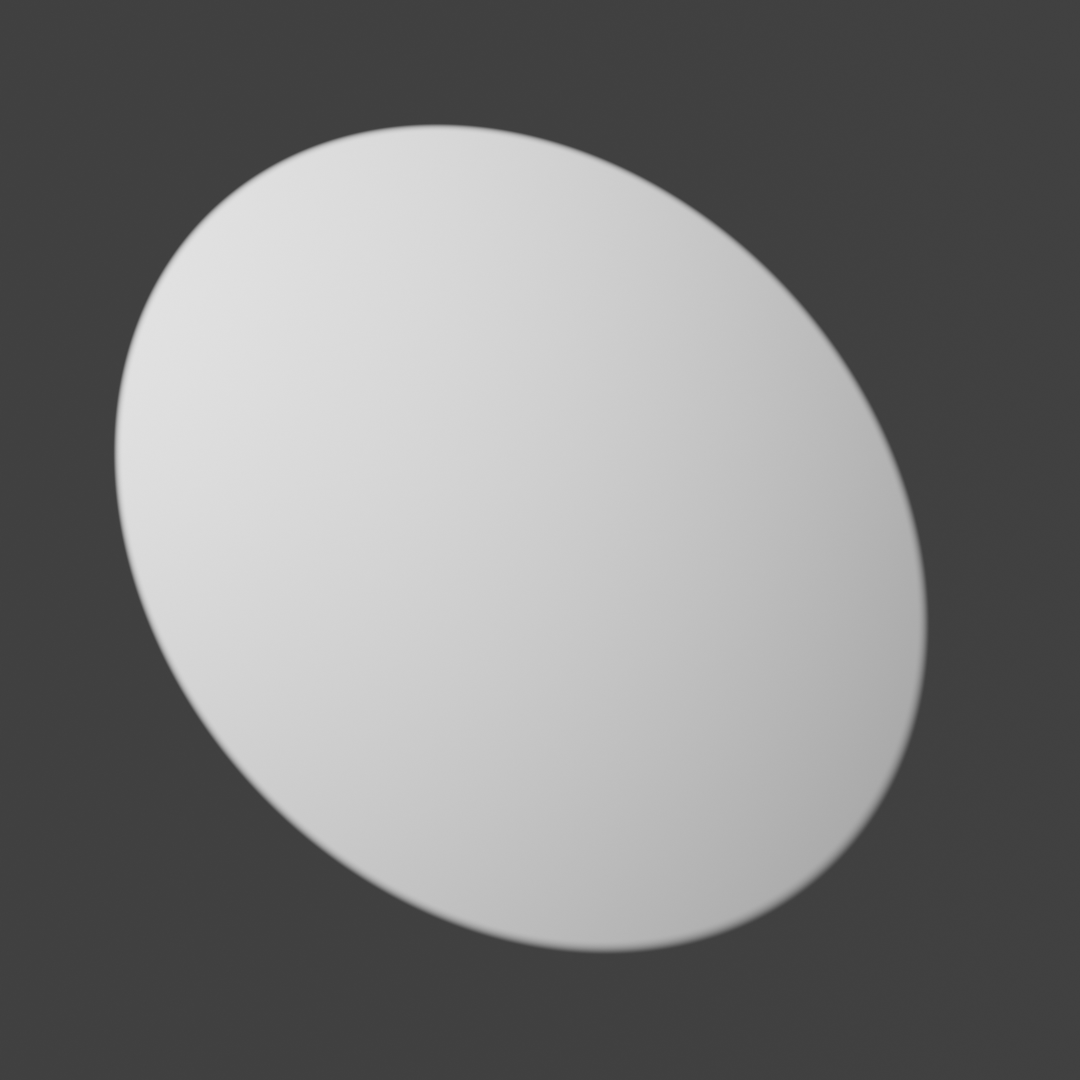
\includegraphics[scale=\myscale,scale=0.1]{figures/spot-02}\quad
	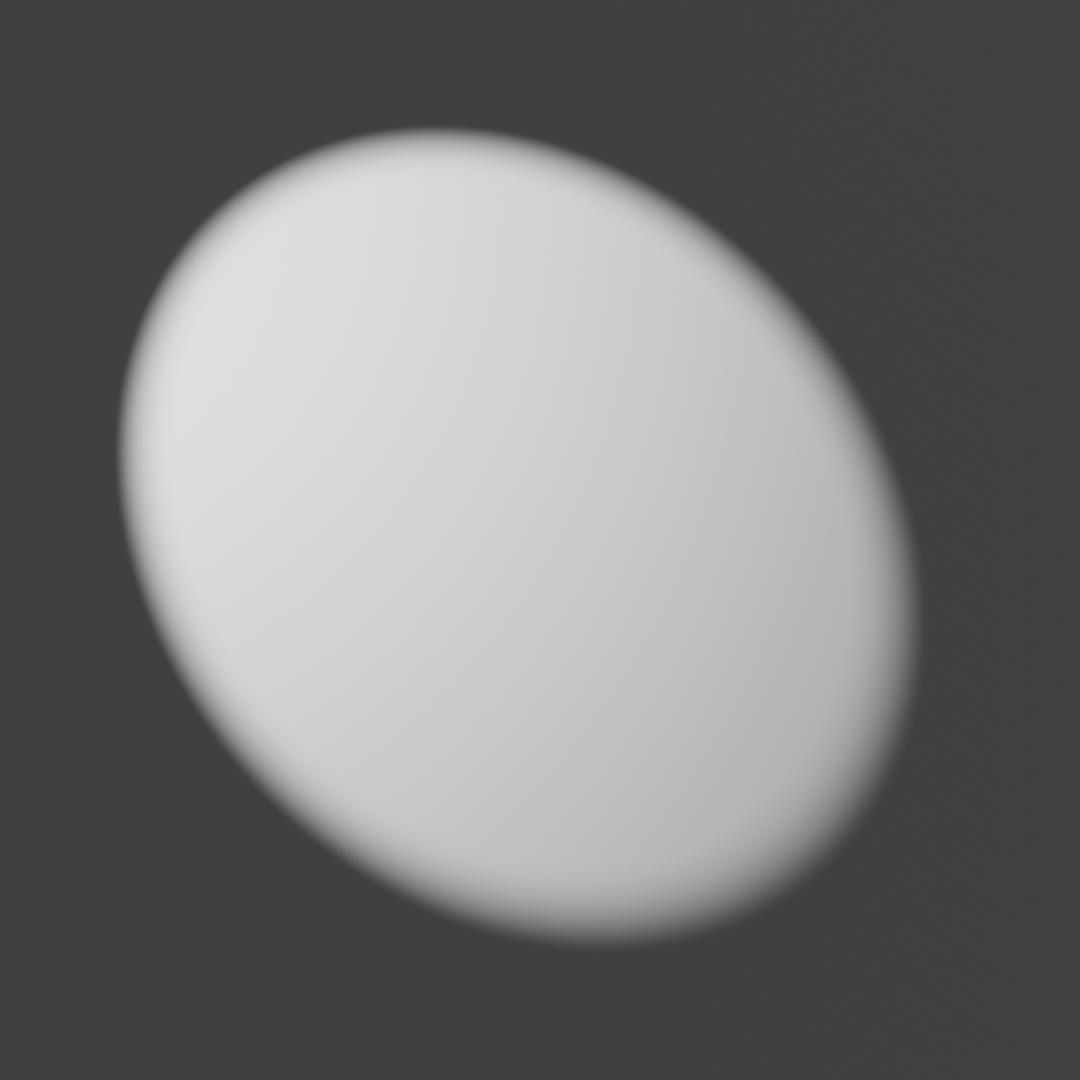
\includegraphics[scale=\myscale,scale=0.1]{figures/spot-03}\quad
	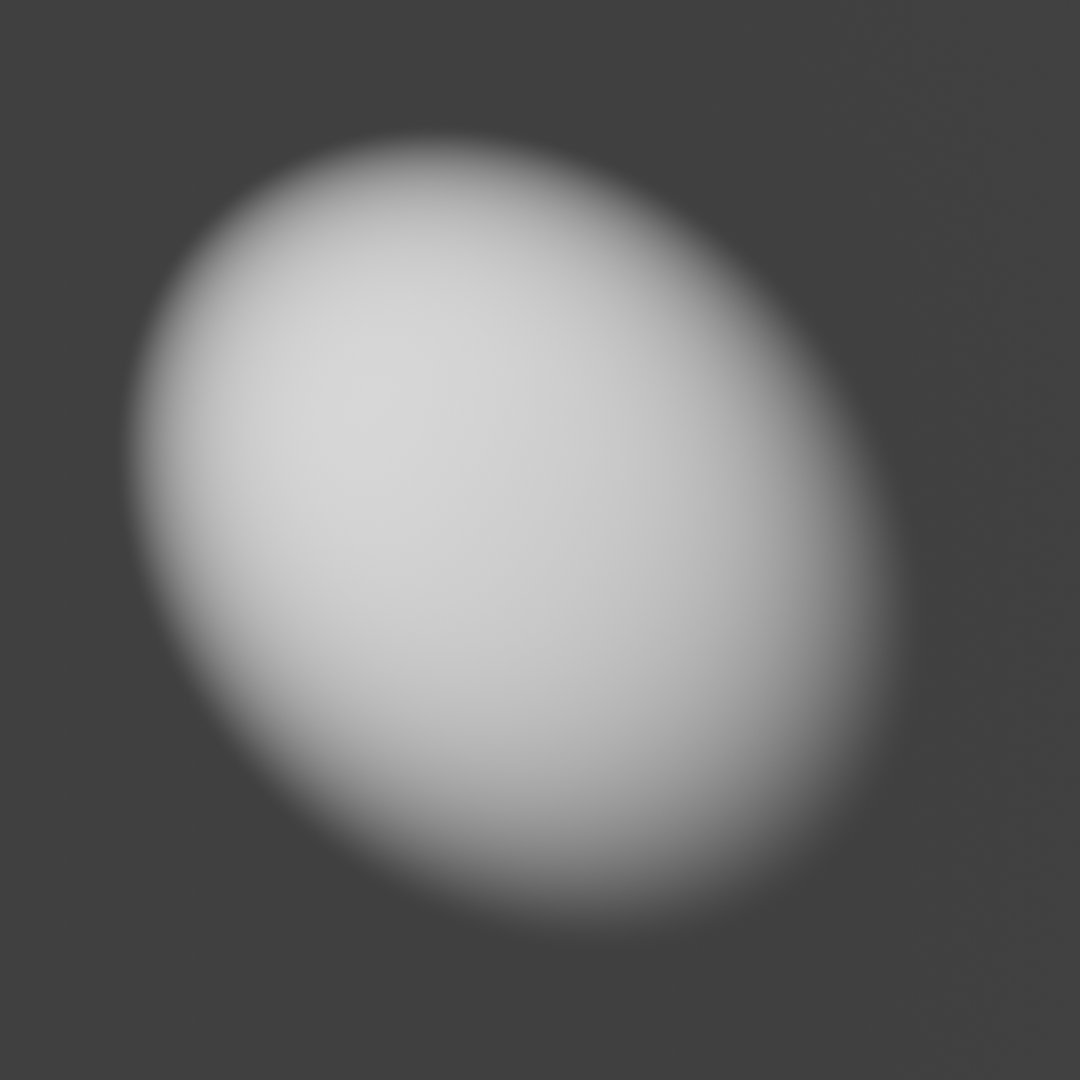
\includegraphics[scale=\myscale,scale=0.1]{figures/spot-04}		
\end{center}


Voici les allures de $\left(\cos(\omega)\right)^{e_\text{att}}$ pour différentes valeurs de l'exposant. Pour $e_\text{att} = 0$ le passage zone éclairée/zone non-éclairée se fait sans transition.
Pour $e_\text{att} > 0$, il y a plateau autour du centre du cône (pour $\omega$ proche de $0$) et une atténuation plus ou moins rapide sur les bords du cône (pour $|\omega|$ proche de $\theta$).

\myfigure{1.2}{\tikzinput{fig-lumiere-11}}
 
Évidemment on peut considérer une version plus générale avec :
$$i_\ell =\frac{1}{\alpha r^2 + \beta r +\gamma} \left(\cos(\omega)\right)^{e_\text{att}}.$$


%%%%%%%%%%%%%%%%%%%%%%%%%%%%%%%%%%%%%%%%%%%%%%%%%%%%%%%%%%%%%%%%%%%%%
\section{Illumination}

%--------------------------------------------------------------------
\subsection{Modèle de Phong}

\index{illumination!de Phong}

La couleur dont est perçu un objet dépend de son éclairage (intensité, direction, couleur\ldots) mais aussi de l'objet lui-même (couleur, matière, brillant/mat\ldots).

Nous modélisons la couleur perçue via le \defi{modèle de Phong}.
Un calcul est à effectuer pour chaque élément de surface.
La couleur s'obtient comme la superposition  de quatre types de luminosité dont on additionne les couleurs :
\begin{itemize}
  \item luminosité irradiante $\Cl_{\text{irr}}$ (facultative),
  \item luminosité ambiante $\Cl_{\text{amb}}$,
  \item luminosité diffuse $\Cl_{\text{diff}}$,
  \item luminosité spéculaire $\Cl_{\text{spec}}$.
\end{itemize}


\begin{center}
	\begin{minipage}{0.32\textwidth}
	\center
	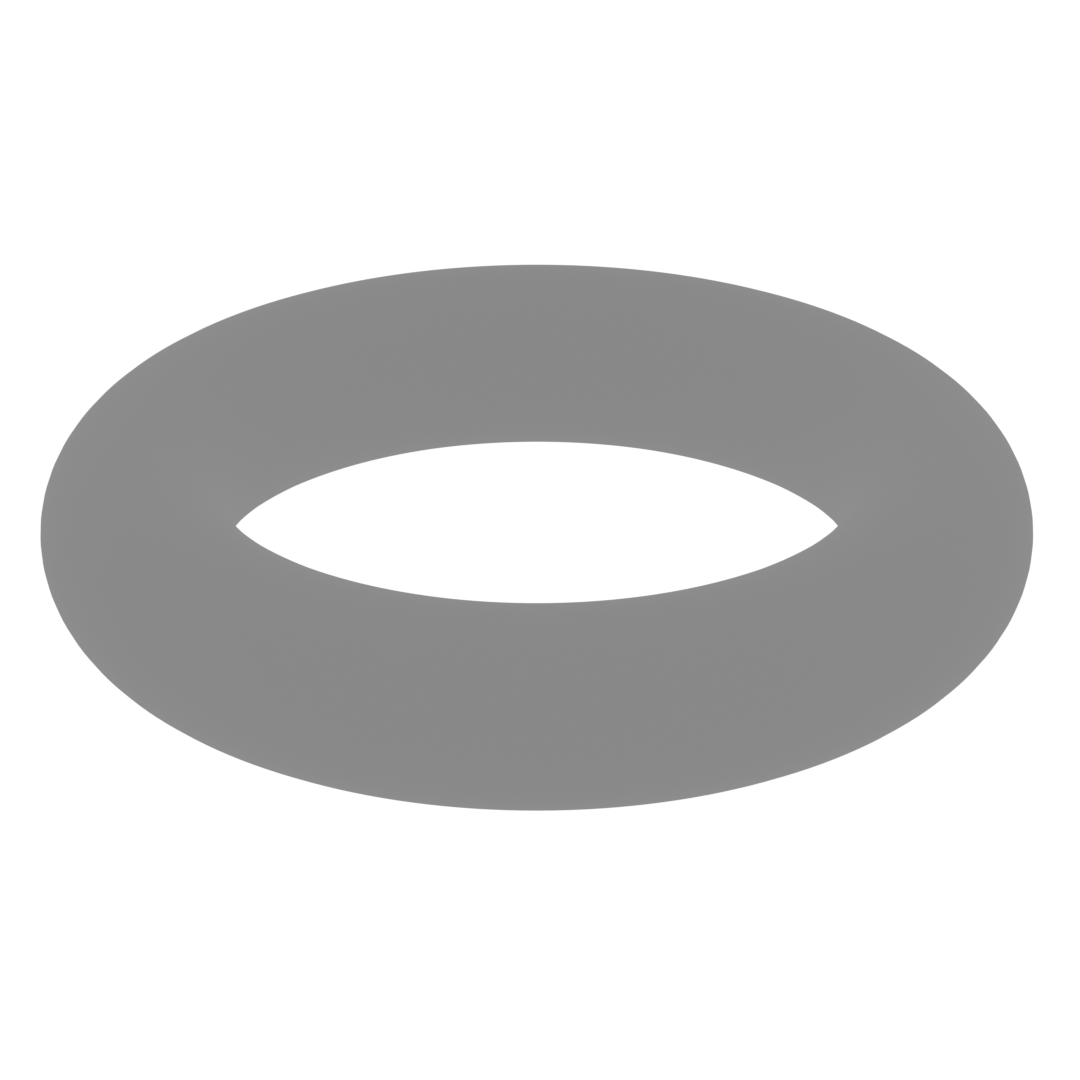
\includegraphics[scale=\myscale,scale=0.15, trim={0 6cm 0 4cm}, clip]{figures/tore-ambiante}
	
	{\bf \qquad Lumière ambiante}
	\end{minipage}
	\begin{minipage}{0.32\textwidth}
	\center
	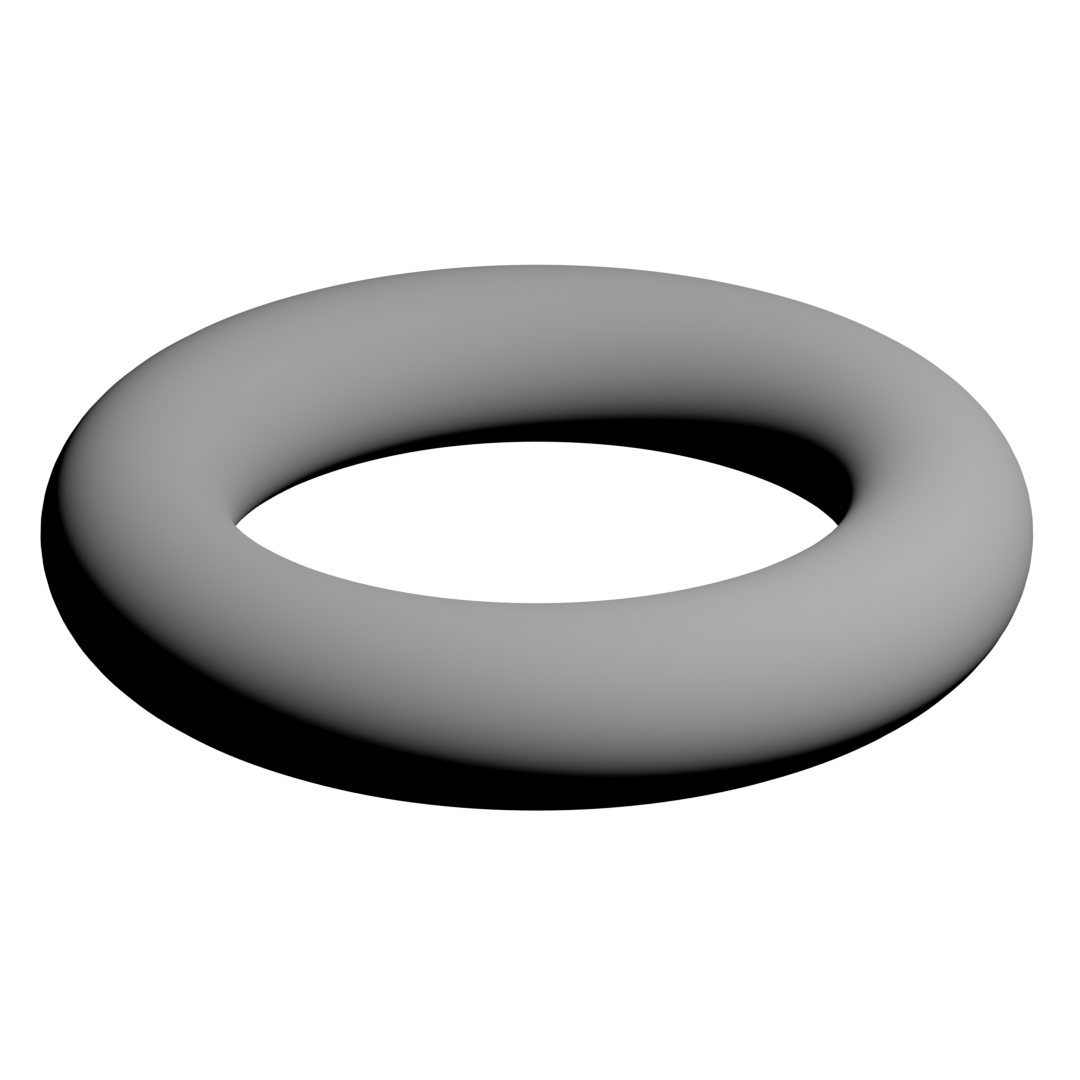
\includegraphics[scale=\myscale,scale=0.15, trim={0 6cm 0 4cm}, clip]{figures/tore-diffuse}
	
	{\bf \qquad Lumière diffuse}
    \end{minipage}
	\begin{minipage}{0.32\textwidth}
	\center
	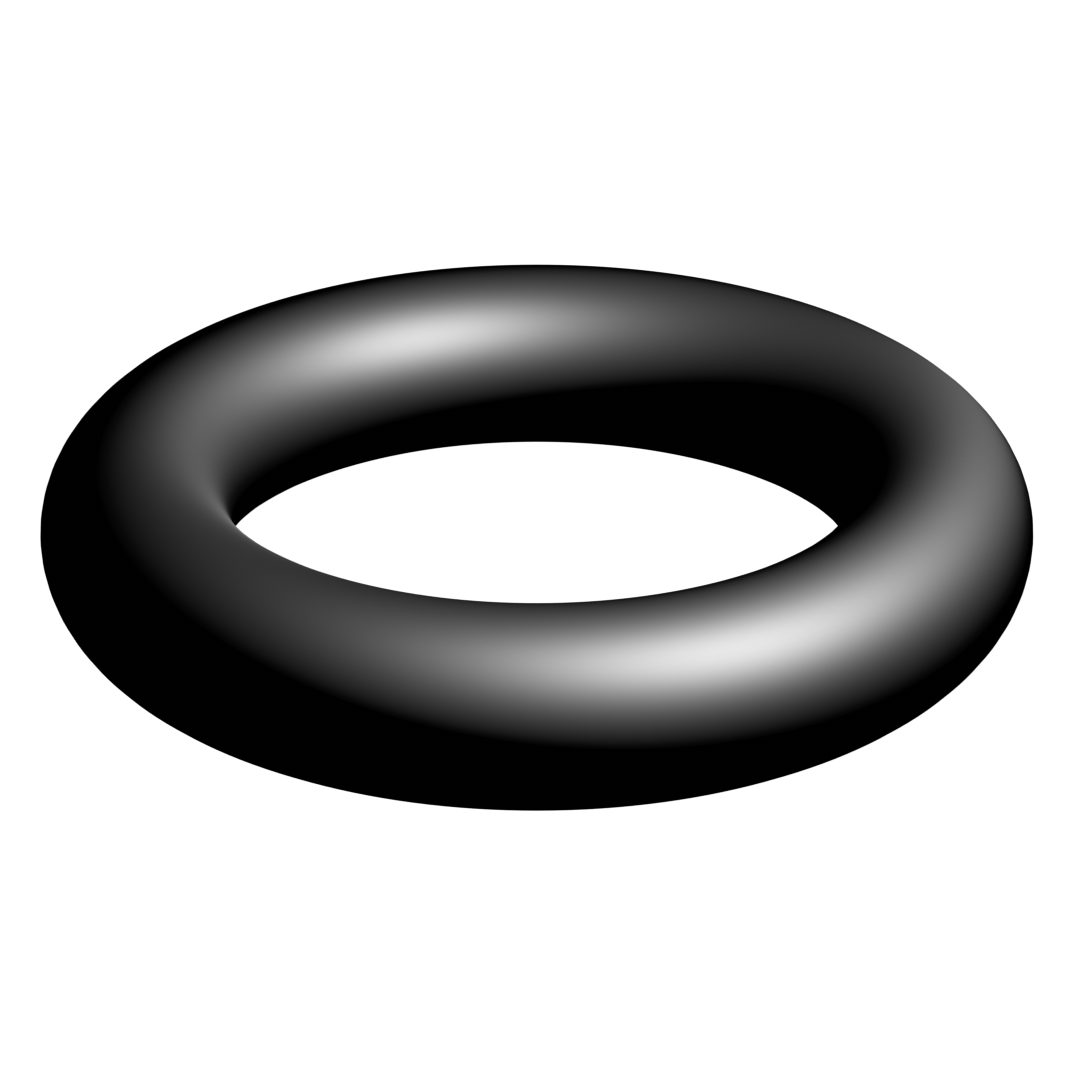
\includegraphics[scale=\myscale,scale=0.15, trim={0 6cm 0 4cm}, clip]{figures/tore-speculaire}
	
	{\bf \qquad Lumière spéculaire}
    \end{minipage}

	\begin{minipage}{0.49\textwidth}
	\center
	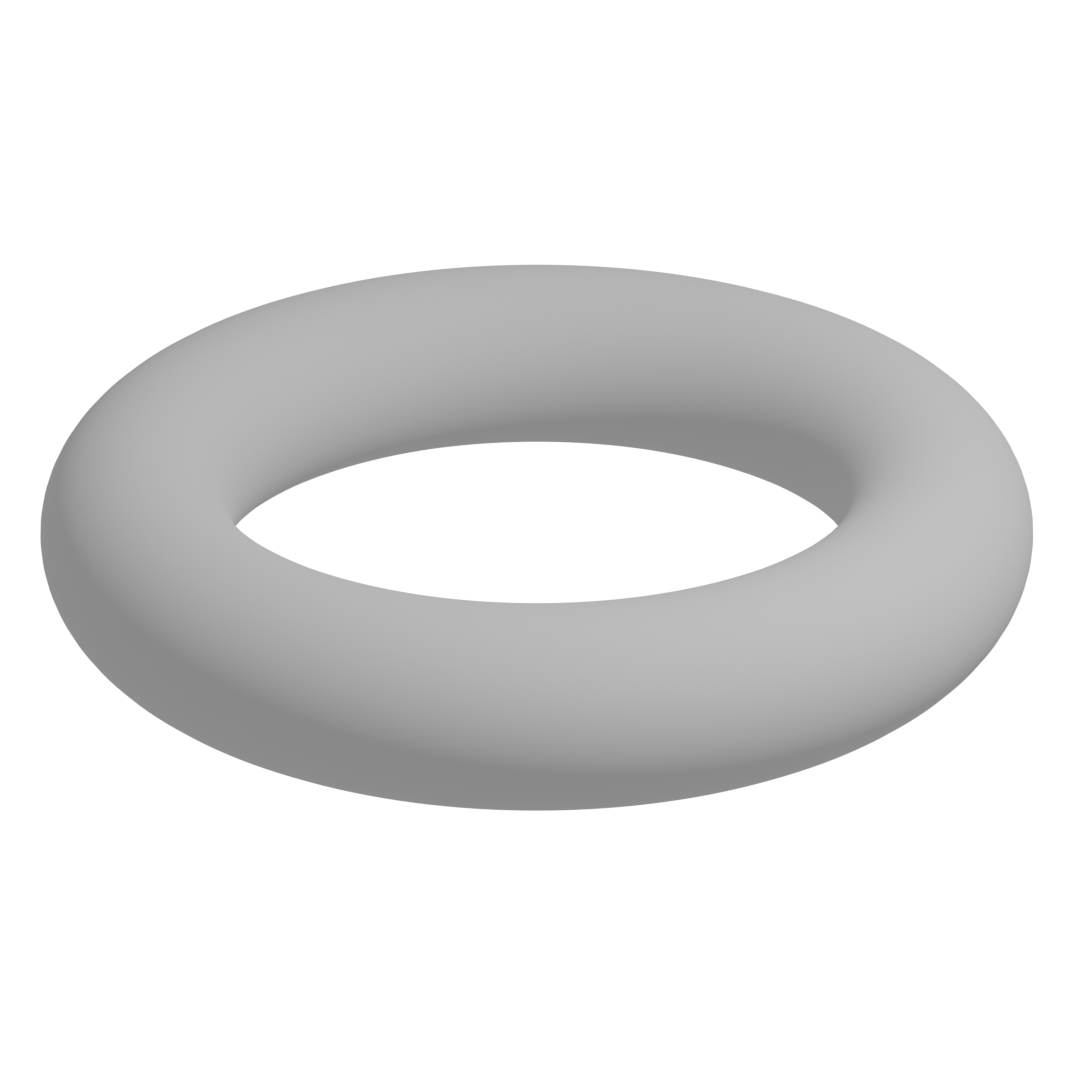
\includegraphics[scale=\myscale,scale=0.20, trim={0 6cm 0 4cm}, clip]{figures/tore-ambiante-diffuse}
	
	{\bf \qquad Lumière ambiante et diffuse}
    \end{minipage}
    \begin{minipage}{0.49\textwidth}
	\center
	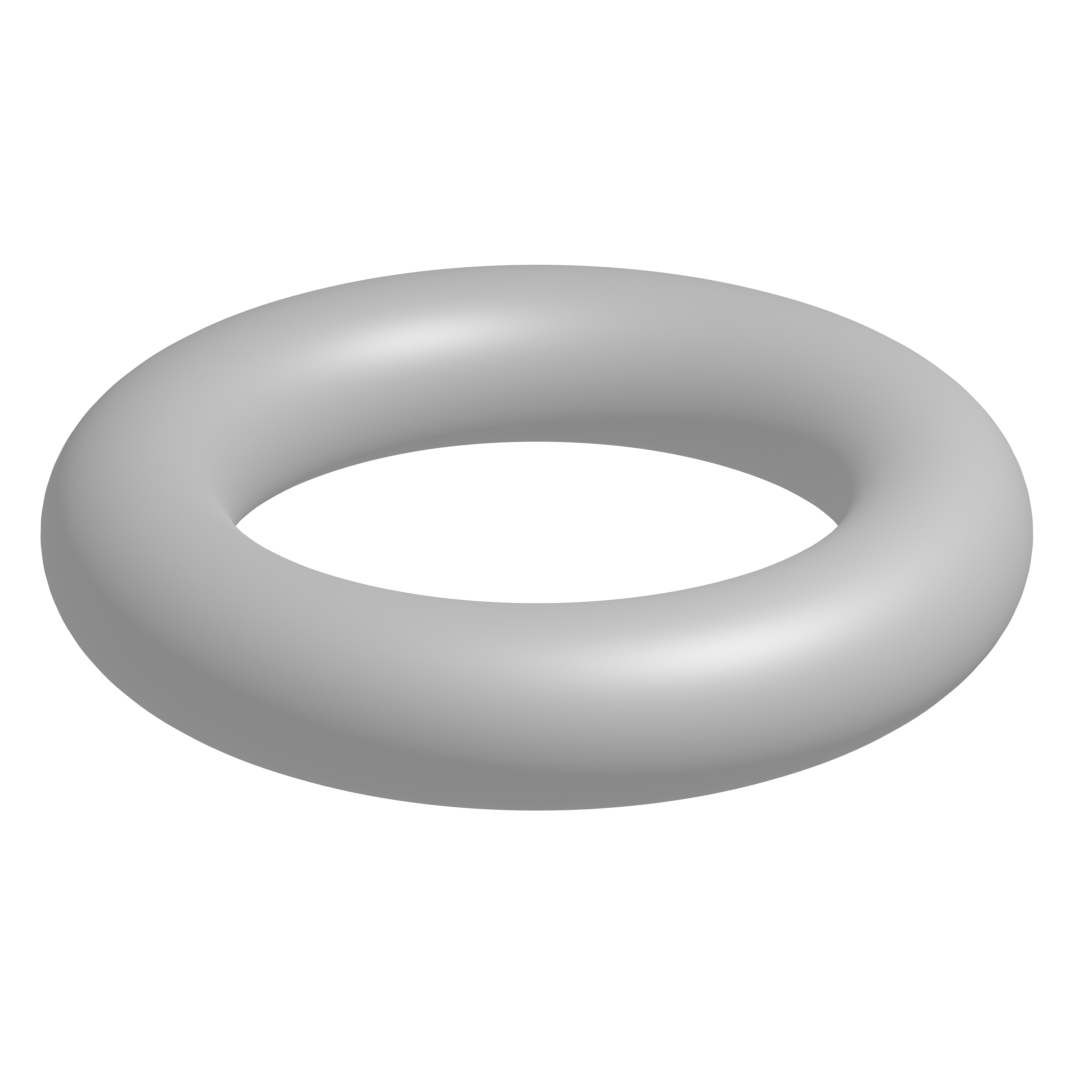
\includegraphics[scale=\myscale,scale=0.20, trim={0 6cm 0 4cm}, clip]{figures/tore-ambiante-diffuse-speculaire}
	
	{\bf \qquad Lumière diffuse, ambiante et spéculaire}
    \end{minipage}
	
\end{center}

La couleur perçue est l'addition de ces couleurs :

\mybox{$\displaystyle \Cl_{\text{perçue}} = \Cl_{\text{irr}} \oplus_{cl} \Cl_{\text{amb}} \oplus_{cl} \Cl_{\text{diff}} \oplus_{cl} \Cl_{\text{spec}}$}

Ce modèle est empirique, et n'est pas fondé sur une réalité physique, mais a fait ses preuves. Il est utilisé dans les moteurs 3D en attendant le \emph{ray-tracing} généralisé.
Nous allons essentiellement considérer une seule source lumineuse (pour plusieurs sources on effectue les calculs pour chaque source et on additionne les résultats). 
Nous omettons ici l'éclairage indirect issu de la réflexion de la lumière sur un autre objet.

\myfigure{0.8}{\tikzinput{fig-lumiere-12}}

%--------------------------------------------------------------------
\subsection{Luminosité irradiante}

La \defi{luminosité irradiante} est une lumière émise par l'objet lui-même, même en l'absence d'éclairage, comme une sorte de rayonnement de l'objet dans toutes les directions. 

\myfigure{0.6}{\tikzinput{fig-lumiere-13}}

La couleur associée est notée : 
\mybox{$\displaystyle \Cl_{\text{irr}}$}
Cette couleur RGB est la même pour tout point de l'objet, quelle que soit la position de l'observateur. 
Cette luminosité est de faible intensité et n'est pas considérée comme une source lumineuse pour les autres objets.



%--------------------------------------------------------------------
\subsection{Luminosité ambiante}

\index{luminosite@luminosité!ambiante}

La \defi{luminosité ambiante} correspond à une lumière qui n'a pas de source précise et éclaire partout, et dans toutes les directions, de la même façon. C'est par exemple le cas d'une scène en extérieur par ciel nuageux, ou bien dans une pièce avec plusieurs fenêtres ayant un voilage. 

\myfigure{0.6}{\tikzinput{fig-lumiere-14}}

La couleur perçue $\Cl_{\text{amb}}$ dépend de la couleur $\Cl_{\text{source}}$ et de l'intensité $i_{\text{source}}$ de l'éclairage, mais aussi de la couleur propre de l'objet $\Cl_{\text{objet}}$ :
\mybox{$\displaystyle \Cl_{\text{amb}} = i_{\text{source}} \Cl_{\text{source}} \otimes_{cl} \Cl_{\text{objet}}$}

Remarques :
\begin{itemize}
  \item On rappelle que $\otimes_{cl}$ désigne la multiplication terme à terme des composantes $r,g,b$.
  
  \item Cette lumière éclaire tous les objets et toutes leurs faces.

  \item C'est un éclairage dont l'intensité reste modérée et qui doit rester discret. Il a pour défaut \og{}d'aplatir\fg{} la scène.

  \item La différence avec la luminosité irradiante est que la luminosité ambiante a une intensité plus forte donc elle pourrait éclairer les autres objets (mais ici nous n'en tiendrons pas compte).
\end{itemize}



%--------------------------------------------------------------------
\subsection{Luminosité diffuse}


\index{luminosite@luminosité!diffuse}

La \defi{luminosité diffuse} est une caractéristique associée aux matériaux mats (ex.: bois, cuir\ldots) dont l'aspect microscopique est rugueux et conduit à une réflexion de la lumière dans toutes les directions.

Voici un zoom à un niveau microscopique d'une surface mate :
\myfigure{0.5}{\tikzinput{fig-lumiere-15}}

La lumière reçue se diffuse dans toutes les directions mais l'intensité diffuse dépend de l'intensité de la lumière reçue et donc de la position de l'objet par rapport à l'éclairage.



\myfigure{0.6}{\tikzinput{fig-lumiere-16}}

La formule de la couleur diffuse est résumée en :
\mybox{$\displaystyle \Cl_{\text{diff}} = i_{\text{source}} \max(\vec\ell\cdot\vec n,0) \Cl_{\text{source}} \otimes_{cl} \Cl_{\text{objet}}$}
où $i_{\text{source}}$ et $\Cl_{\text{source}}$ sont l'intensité et la couleur de la source lumineuse et $\Cl_{\text{objet}}$ est la couleur propre de l'objet.

Expliquons le terme $\max(\vec\ell\cdot\vec n,0)$. Tout d'abord l'éclairage est situé derrière l'objet (autrement dit éclaire la face non visible) lorsque $\vec\ell\cdot\vec n < 0$, dans ce cas $\max(\vec\ell\cdot\vec n,0)=0$ et donc la couleur diffuse est noire $\Cl_{\text{diff}} = (0,0,0)$.

Le produit scalaire $\vec\ell\cdot\vec n$ module l'intensité en fonction de l'orientation de la surface éclairage vis à vis de la source.
Si la surface est perpendiculaire aux rayons lumineux alors $\vec n$ et $\vec \ell$ sont égaux et leur produit scalaire vaut 
$1$. Si la surface n'est pas perpendiculaire, l'intensité est diminuée d'un facteur $\vec\ell\cdot\vec n < 1$.

\medskip

\emph{Justification.}
Considérons l'énergie $E_0$ d'une bande de rayons lumineux de largeur $d$ qui atteint une surface. Dans un premier cas cette surface est perpendiculaire aux rayons et l'énergie $E_0$ se répartit sur une largeur $d$. Dans un second cas la surface est inclinée d'un angle $\theta$, et alors la même énergie $E_0$ se répartit sur une largeur plus grande, égale à $\frac{d}{\cos(\theta)}$.

\myfigure{0.6}{\tikzinput{fig-lumiere-17}}


Si maintenant on raisonne en énergie reçue par unité de surface (par exemple \SI{1}{\meter^2}) alors chaque unité de surface inclinée reçoit moins d'énergie avec un coefficient multiplicatif de $\cos(\theta)$ (qui est inférieur ou égal à $1$).

\myfigure{0.6}{\tikzinput{fig-lumiere-18}}

\medskip

\emph{Remarque.} 
C'est aussi la raison pour laquelle il fait plus froid en hiver qu'en été : en hiver, le Soleil est plus bas dans le ciel et l'énergie reçue s'étale sur une plus grande surface.

\medskip

\emph{Calculs.}
On note $\theta \in ]-\pi,\pi]$ l'angle entre les vecteurs $\vec n$ et $\vec \ell$.
On exprime facilement $\theta$ par la relation :
\mybox{$\cos(\theta) =  \vec \ell \cdot \vec n$}

\begin{center}
\begin{minipage}{0.4\textwidth}
\myfigure{0.6}{\tikzinput{fig-lumiere-19}}
\end{minipage}\qquad
\begin{minipage}{0.4\textwidth}
\myfigure{0.6}{\tikzinput{fig-lumiere-20}}
\end{minipage}
\end{center}

Et les relations trigonométriques usuelles, montrent que la bande de largeur $d$ illumine sur la surface inclinée une bande de largeur $\frac{d}{\cos(\theta)}$.
Par conséquence l'intensité lumineuse diffuse s'exprime par :
$$i_{\text{diff}} =  i_{\text{source}} \times \cos(\theta) = i_{\text{source}} \; \vec \ell \cdot \vec n.$$

Cela explique presque complètement les termes de la formule. Cependant on ne diffuse pas de lumière si la source est derrière l'objet, c'est-à-dire si $|\theta| > \frac\pi2$ (dans ce cas la lumière arrive sur la face cachée). Or, pour nos angles, 
$|\theta| > \frac\pi2$ équivaut à $\cos(\theta) < 0$, donc si $\cos(\theta) < 0$ on fixe $i_{\text{diff}} = 0$.

\myfigure{0.5}{\tikzinput{fig-lumiere-21}}

Résumons :
$$i_{\text{diff}} =  i_{\text{source}} \max(0,\cos(\theta)) = 
\begin{cases}
i_{\text{source}}\cos(\theta) & \text{si }\cos(\theta) \ge 0,\\
0 & \text{sinon.}
\end{cases}$$


%--------------------------------------------------------------------
\subsection{Luminosité spéculaire}

\index{luminosite@luminosité!speculaire@spéculaire}

La luminosité diffuse vue précédemment renvoie uniformément la lumière dans toutes les directions. Mais en réalité, la lumière se réfléchit davantage par réflexion sur la surface : c'est la \defi{luminosité spéculaire}.
Elle s'observe sur les objets brillants (plastique, métal poli\ldots), le cas extrême étant celui d'un miroir sur lequel un rayon lumineux est renvoyé dans une seule direction. Cependant, si la surface est moins lisse, les réflexions s'étalent autour d'une direction privilégiée (la distribution étant centrée autour d'un axe principal de réflexion).


\myfigure{0.5}{\tikzinput{fig-lumiere-22}}

Attention ! La luminosité spéculaire perçue dépend de la position de l'observateur. Elle demande donc davantage de calculs que les luminosités précédentes. Par contre elle apporte une grosse touche de réalisme.

Notons $\vec r$ l'axe principal de la réflexion, qui est le vecteur symétrique de $\vec\ell$ (qui pointe vers la source lumineuse $S$) par rapport à $\vec n$ (orthogonal à la surface). Notons $\vec{v}$ le vecteur, issu de $P$, pointant vers l'observateur $O$.
Nous supposons que $\vec{\ell}$, $\vec{n}$, $\vec{r}$, $\vec{v}$ sont des vecteurs unitaires.


\myfigure{0.5}{\tikzinput{fig-lumiere-23}}

\begin{lemme}
\label{lem:vecr}
\sauteligne
\mybox{$\vec r = 2(\vec \ell \cdot \vec n) \vec n - \vec\ell$}
\end{lemme}


Voici la formule de la couleur de la luminosité spéculaire.

Si $\vec\ell \cdot \vec n \ge 0$ et $\vec r \cdot \vec v \ge 0$ alors :
\mybox{$\displaystyle \Cl_{\text{spec}} 
= i_{\text{source}} \; (\vec r\cdot\vec v)^{e_{\text{spec}}} \;
\Cl_{\text{source}} \otimes_{cl} \Cl_{\text{objet}} $}

Si $\vec\ell \cdot \vec n < 0$ ou $\vec r \cdot \vec v < 0$ alors, la surface n'est pas visible ou pas éclairée et on pose :
$$\displaystyle \Cl_{\text{spec}} = (0,0,0)$$


\myfigure{0.6}{\tikzinput{fig-lumiere-24bis}}

La formule dépend :
\begin{itemize}
  \item de $i_{\text{source}}$ et $\Cl_{\text{source}}$ : l'intensité et la couleur de la source lumineuse,
  \item de la position de l'axe principal de réflexion $\vec r$ par rapport à la direction $\vec v$ vers l'observateur,
  \item d'un exposant $e_{\text{spec}}$ qui est un paramètre d'étalement,
  \item et de $\Cl_{\text{objet}}$, la couleur propre de l'objet.
\end{itemize}

\myfigure{0.6}{\tikzinput{fig-lumiere-24}}

\bigskip

\emph{Justifications.}

\textbf{Preuve du lemme \ref{lem:vecr}.}
\begin{proof}
Notons $\vec p$ un vecteur orthogonal à $\vec n$, appartenant au plan $(P,\vec n,\vec \ell)$. 
\myfigure{0.5}{\tikzinput{fig-lumiere-25}}

Dans la base $(\vec n, \vec p)$, écrivons :
\begin{equation}
\label{eq:vecl}
\vec \ell = \alpha \vec n + \beta \vec p
\end{equation}
Alors, par symétrie, on aura :
$$\vec r = \alpha \vec n - \beta \vec p.$$

\emph{Calcul de $\alpha$.} On effectue le produit scalaire des termes de l'égalité \eqref{eq:vecl} avec $\vec n$ :
$$\vec \ell \cdot \vec n = \alpha \vec n \cdot \vec n + \beta \vec p  \cdot \vec n,$$
donc 
$$\vec \ell \cdot \vec n = \alpha \cdot 1 + \beta \cdot 0.$$
Ainsi $\alpha = \vec \ell \cdot \vec n$.

\emph{Calcul de $\vec r$.} On repart de l'égalité \eqref{eq:vecl} :
$$\beta \vec p = \vec \ell - \alpha \vec n,$$
donc
$$\vec r 
= \alpha \vec n - \beta \vec p 
= \alpha \vec n -(\vec \ell - \alpha \vec n)
= 2\alpha \vec n - \vec\ell 
= 2(\vec \ell \cdot \vec n) \vec n - \vec\ell.$$

\end{proof}

\medskip
\textbf{Calcul de l'angle $\omega$.}
Notons $\omega$ l'angle entre $\vec v$ (dirigé vers l'observateur) et $\vec r$ (axe principal de réflexion). 

\myfigure{0.7}{\tikzinput{fig-lumiere-26}}

Alors :
$$\cos(\omega) = \vec r \cdot \vec v.$$

\medskip
\textbf{Intensité réfléchie/perçue.}
L'intensité renvoyée par réflexion dépend de l'angle $\omega$, elle diminue lorsque l'observateur s'éloigne de l'axe principal de réflexion, selon la formule :
$$(\cos(\omega))^{e_{\text{spec}}}$$
Plus l'exposant est grand, plus l'intensité lumineuse se concentre autour de l'axe principal de réflexion.

\myfigure{1}{\tikzinput{fig-lumiere-27}}


\medskip
\textbf{Validité des formules.}

D'une part, on souhaite éclairer la face visible, donc il faut $\vec \ell \cdot \vec n \ge 0$. D'autre part, l'observateur doit être du \og{}bon\fg{} côté de la réflexion, c'est-à-dire $\vec r \cdot \vec v \ge 0$. Dans les autres cas, la lumière atteint une face cachée ou bien n'est pas du tout renvoyée vers l'observateur.

\bigskip
\emph{Lumière diffuse/lumière spéculaire.}
Un même éclairage peut avoir une composante diffuse et une composante spéculaire, on distingue alors deux intensités $i_{\text{source,diff}}$ et $i_{\text{source,spec}}$.

Voici un exemple de combinaison de ces deux composantes : à gauche les luminosités diffuses et spéculaires séparées, à droite la lumière résultante.
\myfigure{0.6}{\tikzinput{fig-lumiere-28}}

\medskip
\textbf{Variante Blinn--Phong.}

\index{illumination!de Blinn-Phong}

Comme on l'a dit, la lumière spéculaire nécessite beaucoup de calculs car il faut à chaque fois calculer le vecteur $\vec v$ qui dépend de $C$ et de $P$, mais aussi le vecteur $\vec r$.

Il existe une variante pour la formule de la luminosité spéculaire, appelée \defi{variante Blinn--Phong}. Certains trouvent le rendu un peu plus réaliste, et elle a l'avantage de demander moins de calculs dans certaines situations.

Définissons le \defi{vecteur bissecteur} (\emph{half-way vector}) : 
$$\vec h = \frac{\vec \ell + \vec v}{\|\vec \ell + \vec v\|}.$$

\myfigure{0.7}{\tikzinput{fig-lumiere-29}}

La nouvelle formule est alors :
\mybox{$\displaystyle Cl'_{\text{spec}} 
= i_{\text{source}} (\vec h\cdot\vec n)^{e'_{\text{spec}}}  
\Cl_{\text{source}} \otimes_{cl} \Cl_{\text{objet}} $}
valide lorsque  $\vec\ell \cdot \vec n \ge 0$ et $\vec h \cdot \vec n \ge 0$.

Il faut ajuster l'exposant $e'_{\text{spec}}$ pour retrouver des effets similaires à la formule classique.

Expliquons l'avantage de la formule de Blinn-Phon. Si on considère un éclairage directionnel, c'est-à-dire où $\vec\ell$ est un vecteur constant et un observateur éloigné, c'est-à-dire $\vec v$ est aussi un vecteur constant, alors le vecteur bissecteur $\vec h$ est un vecteur constant (indépendant de l'objet) et n'a besoin d'être calculé qu'une seule fois, pour calculer le produit scalaire  $\vec h\cdot\vec n$. Par contre dans la formule classique, le calcul de $\vec r \cdot \vec v$ nécessite au préalable le calcul de $\vec r$, qui varie pour chaque surface élémentaire (via $\vec n$).


\end{document}
